\documentclass[12pt, a4paper]{article}
% MARGÓK
\usepackage[margin=2.5cm]{geometry} 

% SORKÖZ
\usepackage{setspace}
\onehalfspacing

\usepackage{graphicx}
\usepackage{textcomp}
\usepackage[hungarian]{babel}
\usepackage[T1]{fontenc}
\usepackage[utf8]{inputenc}
\usepackage{caption}
\usepackage{subcaption}
\usepackage{csquotes}
\graphicspath{{./Pictures/}}
\usepackage[style=ieee]{biblatex}
\addbibresource{onlab.bib}

\usepackage{listings}
\usepackage[svgnames]{xcolor}
\usepackage{tikz}
\usetikzlibrary{shapes.geometric, arrows, calc}

\usepackage{float}
\usepackage{amsmath}
\usepackage{tabularx}
\usepackage{url}


% ... többi csomag (graphicx, babel, stb.) ...

% Színbeállítások kódkiemeléshez
\definecolor{dkgreen}{rgb}{0,0.6,0}
\definecolor{gray}{rgb}{0.5,0.5,0.5}
\definecolor{mauve}{rgb}{0.58,0,0.82}

\lstset{frame=none,
  language=Bash,
  aboveskip=3mm,
  belowskip=3mm,
  showstringspaces=false,
  columns=flexible,
  basicstyle={\small\ttfamily},
  numbers=none,
  numberstyle=\tiny\color{gray},
  keywordstyle=\color{blue},
  commentstyle=\color{dkgreen},
  stringstyle=\color{mauve},
  breaklines=true,
  breakatwhitespace=true,
  tabsize=2
}

% TikZ stílusok
\tikzstyle{box} = [rectangle, rounded corners, minimum width=3cm, minimum height=0.5cm,text centered, draw=black, fill=orange!30]
\tikzstyle{arrow} = [thick,->,>=stealth]

% --- CÍMOLDAL ADATOK ---
\title{\textbf{Audio tömörítő egység megvalósítása FPGA-val}}
\author{Nyiri Levente}
\date{2025 Október}

\begin{document}

% -------------------------------------------------------------------------
% 1. CÍMOLDAL
% -------------------------------------------------------------------------
\begin{titlepage}
    \centering
    
\includegraphics[width=0.8\textwidth]{BME.png} 
    \vspace{1cm}
    
    {\Huge \textbf{Audio tömörítő egység megvalósítása FPGA-val} \par}
    
    \vspace{2cm}
    
    {\large Önálló laboratórium 2. zárójegyzőkönyv \par}
    {\large 2025/26. I. félév \par}
    \vspace{3cm}
    
    {\Huge \textbf{Nyiri Levente (ULYHQH)} \par}
    \vspace{0.5cm}
    {\large Villamosmérnök szakos hallgató \par}
    {\large MSc FPGA alapú rendszerek mellékspecializáció \par}
    \vspace{2cm}
    
    {\large Konzulens: \par}
    \vspace{0.5cm}
    {\large Szántó Péter \par}
    {\large (Mesterséges Intelligencia és Rendszertervezés Tanszék) \par}
    
    \vspace{2cm}
\end{titlepage}

\selectlanguage{hungarian}

% -------------------------------------------------------------------------
% 2. FELADATKIÍRÁS
% -------------------------------------------------------------------------
\newpage
\section*{Feladatkiírás}
Az AMD Ultrascale+ MPSoC FPGA-k használata számos multimedia feldolgozást igénylő alkalmazásban kedvező opció. 

Míg a video tömörítésre az eszköz dedikált hardver egységet tartalmaz, addig az audio kezelése elsősorban az általános célú ARM processzoros alrendszeren oldható meg. Ez azonban fogyasztás, illetve CPU terhelés szempontjából nem feltétlenül optimális.

A feladat célja, az alkalmazások jelentős részében előkerülő audio tömörítésre egy, az FPGA általános erőforrásait felhasználó hardver gyorsító kifejlesztése, valamint ennek összehasonlítása a tisztán szoftveres megoldással.

% -------------------------------------------------------------------------
% 3. TARTALOMJEGYZÉK
% -------------------------------------------------------------------------
\newpage
\tableofcontents
\newpage

% -------------------------------------------------------------------------
% 4. BEVEZETÉS
% -------------------------------------------------------------------------
\section{Bevezetés}
% A feladat értelmezése, a specifikáció pontosítása

A dolgozat célja bemutatni egy FPGA alapú audio tömörítő rendszer tervezési lépéseit. A munkát ebben a félévben kezdtem, és a feladat komplexitásából kifolyólag várhatóan a Diplomatervezés 2. tárgy keretén belül fogom befejezni.

\section{Technológiai háttér}

Veszteséges tömörítés mellett döntöttem, tanulmányoztam az MPEG-1 Audio és az MPEG-2 Advanced Audio Coding (AAC) szabványokat, úgy döntöttem, hogy az MPEG-1 Audio Layer III(MP3)-at fogom implementálni.

Bár az AAC egy modernebb szabvány, az MP3 továbbra is széles körben használatban van, viszont több segédanyag található hozzá, ami megkönnyíti a fejlesztést. Ezen okból kifolyólag MP3 encoder-t fogok megvalósítani.

Több open source MP3 encoder is létezik, a legnépszerűbb a LAME, ezt fogom használni, hogy összevessem az FPGA-s megvalósítást a szoftveressel.

A szabvány megértéséhez többek közt a LAME forrás kódját is olvastam, illetve lefordítottam és kipróbáltam egy test .wav file-al.


% -------------------------------------------------------------------------
% 6. A TERVEZÉS RÉSZLETES LEÍRÁSA
% -------------------------------------------------------------------------
\section{Encoder}
% A választott megoldások indoklása

Az encoder egyszerűsített blokkvázlata\cite{mp3-iso} az \ref{fig:encoder-diagram}. ábrán látható.

\begin{figure}[H]
  \centering
  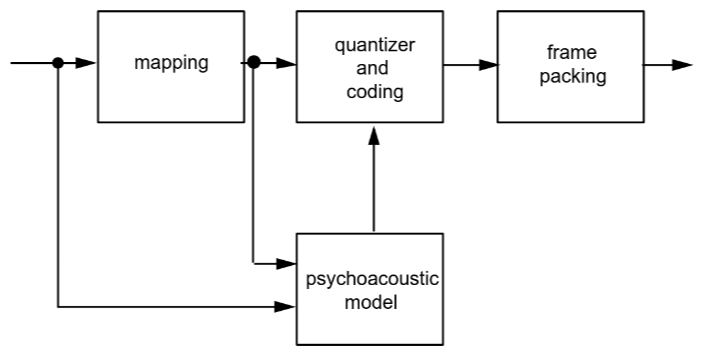
\includegraphics[width=0.8\textwidth]{encoder-diagram.png}
  \caption{Encoder blokkvázlat}
  \label{fig:encoder-diagram}
\end{figure}

\subsection{Frame struktúra}

Egy MP3 file kisebb részegységekre van osztva, ezeket frame-eknek hívjuk. Minden frame 1152 audio mintát tartalmaz. Egy frame továbbá szét van választva 2 granule-ra, mindkettőre 576 minta jut.
Egy frame méretét byteban a(z) \ref{eq:frame-size}. egyenlet írja le.   

\begin{equation}
    \label{eq:frame-size}
    \text{frame size} = \frac{144 \cdot \text{bitrate}}{f_s} + \text{Padding}
\end{equation}
Egy frame felépítése a(z) \ref{tab:frame-header}. táblázatban \cite{raissi-mp3} látható.

\begin{table}[h]
\centering
\begin{tabular}{|c|c|c|c|c|}
  \hline
  \texttt{Header} & \texttt{CRC} & \texttt{Side\_Information} & \texttt{Main\_Data} & \texttt{Ancillary\_Data} \\
  \hline
\end{tabular}
\caption{Az MPEG-1 Audio frame mezői}
\label{tab:frame-header}
\end{table}

\subsubsection{Header}
A header tartalmazza a szinkronizációs biteket és egyéb információkat a frame-ről, felépítését mutatja a(z) \ref{fig:frame-header}. ábra \cite{raissi-mp3}.

\begin{figure}[H]
  \centering
  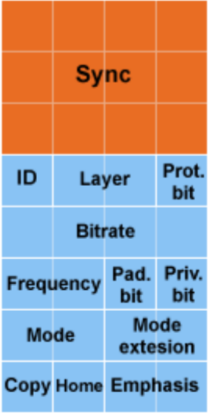
\includegraphics[width=0.2\textwidth]{frame-header.png}
  \caption{Frame header}
  \label{fig:frame-header}
\end{figure}

\begin{description}
  \item[Sync (12 bit)] Szerepe a szinkronizálás, mind a 12 bitnek 1-esnek kell lennie: \texttt{sync = 12'b1111\_1111\_1111}
  \item[ID (1 bit)] Az MPEG verziót határozza meg (MPEG-1 vagy MPEG-2)
  \item[Layer (2 bit)] Layer I, II vagy III 
  \item[Protection bit (1 bit)] Meghatározza, használunk-e CRC-t
  \item[Bitrate (4 bit)] A bitrate beállítása
  \item[Frequency (2 bit)] A mintavételi frekvencia meghatározása
  \item[Padding bit (1 bit)] Néhány frame-nek szüksége van rá, hogy a bitrate pontos legyen
  \item[Private bit (1 bit)] Applikáció-specifikus trigger
  \item[Mode (2 bit)] Csatornamód 
  \item[Mode extension (2 bit)] Csak joint stereo esetén használatos, további specifikáció
  \item[Copyright bit (1 bit)] Jelzi, ha a tartalom szerzői jogi védelem alatt áll
  \item[Home bit (1 bit)] A frame az eredeti adathordozón található-e
  \item[Emphasis (2 bit)] A dekódernek szükséges-e de-emphasist alkalmaznia zajcsökkentés után
\end{description}

\vspace{0.5cm} 
\noindent \textbf{Megkötések:}
\vspace{0.5cm} 

Mivel egy általános, minden opciót támogató encoder túlmutat a feladat keretein, a tervezés során a(z) \ref{tab:bit-constraints}. táblázatban látható fix konfigurációs beállításokat alkalmazom a Header mezőire vonatkozóan.

\begin{table}[h]
\centering
\footnotesize
\begin{tabular}{|c|c|p{6cm}|}
  \hline
  \textbf{Mező Neve} & \textbf{Bit Érték} & \textbf{Jelentés} \\
  \hline
   ID & 1 & MPEG-1 \\
  \hline
  Layer & 01 & Layer III \\
  \hline
  Protection bit & 1 & Használunk CRC-t \\
  \hline
  Bitrate & 1110 & 320 Kbps \\
  \hline
  Frequency & 00 & 44.1 kHz mintavételi frekvencia \\
  \hline
  Mode & 00 & Stereo \\
  \hline
  Emphasis & 00 & Nem kell de-emphasis dekódolásnál, nem használunk noise suppression-t \\
  \hline
\end{tabular}
\caption{Megkötések a bitekre}
\label{tab:bit-constraints}
\end{table}

\subsubsection{Side information}

A side information további információt tartalmaz arra vonatkozóan, hogy hogyan kell dekódolni a frame-et. A felépítését a(z) \ref{tab:side-info}. táblázat mutatja.

\begin{table}[h]
\centering
\footnotesize
\begin{tabular}{|c|c|c|c|c|}
  \hline
  \texttt{main\_data\_begin} & \texttt{private\_bits} & \texttt{scfsi} & \texttt{Side\_info gr. 0} & \texttt{Side\_info gr. 1} \\
  \hline
\end{tabular}
\caption{A side information mezői}
\label{tab:side-info}
\end{table}

\begin{description}
  \item [main\_data\_begin (9 bit)] Layer III-nál bit reservoir használatával egy adott frame main data helyén szabadon maradt helyet másik frame-ek is használhatják. Ez a mező azt a negatív offsetet adja meg, amennyivel korábban kezdődik egy frame-nek a main data-ja a sync word-höz képest.
  \item [private\_bits (5 bit)] Szabad felhasználás 
  \item [scfsi (4-4 bit)] ScaleFactor Selection Information, azt határozza meg, hogy az egyes scalefactor-ok mindkét granule-ra használhatóak-e vagy külön kell mindkettőre küldeni. Ha elég csak egyet küldeni, azzal biteket nyerünk, amit Huffman kódoláshoz lehet használni.
  
  Layer III-nál a scalefactorok 4 csoportba vannak osztva a(z) \ref{tab:scalefactor-bands}. táblázat szerint. Mindkét csatornára vonatkozóan, ha egy bit 1-esbe van, akkor az adott csoporthoz tartozó scalefactorokat a frameben lévő második granule újra fogja használni. Ha short window-t használunk (block\_type == 2) bármely granule-ban, akkor a scalefactorokat mindig külön küldjük mindkét csatornára.
  
  \begin{table}[h]
  \centering
  \footnotesize
  \begin{tabular}{|c|c|}
    \hline
    \textbf{group} & \textbf{scalefactor bands} \\
    \hline
    0 & 0,1,2,3,4,5 \\
    \hline
    1 & 6,7,8,9,10 \\
    \hline
    2 & 11,12,13,14,15 \\
    \hline
    3 & 16,17,18,19,20 \\
    \hline
  \end{tabular}
  \caption{Scalefactor csoportok}
  \label{tab:scalefactor-bands}
  \end{table}
\end{description}

A granule-okhoz tartozó \texttt{side\_info} még további mezőkből áll, ezt mutatja a(z) \ref{tab:granule-side-info}. táblázat.

\begin{table}[h]
\centering
\footnotesize
\begin{tabular}{|l|l|l|l|}
  \hline
  \texttt{part2\_3\_length} & \texttt{big\_values} & \texttt{global\_gain} & \texttt{scalefac\_compress} \\
  \hline
  \texttt{windows\_switching\_flag} & \texttt{block\_type} & \texttt{mixed\_block\_flag} & \texttt{table\_select} \\
  \hline
  \texttt{subblock\_gain} & \texttt{region0\_count} & \texttt{region1\_count} & \texttt{preflag} \\
  \hline
  \texttt{scalefac\_scale} & \texttt{count1table\_select} & \multicolumn{2}{c}{} \\
  \cline{1-2}
\end{tabular}
\caption{Granule side information mezői}
\label{tab:granule-side-info}
\end{table}

\begin{description}
  \item [par2\_3\_length (12-12 bit)] Megmondja, hogy a main data részében a frame-nek hány bit van allokálva scalefactor-oknak (part2) és Huffman kódolt adatnak (part3).
  \item [big\_values (9-9 bit)] Az egyes granule-ok spektrális komponensei más Huffman kód táblázatokkal vannak kódolva. A teljes spektrum 0-tól a Nyquist frekvenciáig több részre van bontva, és ezek a részek máshogy vannak kódolva. A partícionálás a maximális kvantált értékek alapján történik. 
  
  Megszámoljuk, hogy minden frekvencián összesen hány 0 érték van, ezeknek a számát az \texttt{rzero}-ban tároljuk. A \texttt{count1} mezőben 4-esével vannak értékek, és az abszolútértéke nem haladja meg az 1-et. A többi érték a \texttt{big\_values} mezőben van, ezen belül is 3 részre osztva. Az abszolút maximum értéke ennek a régiónak 8191.
    
    A big\_values mező felosztása a(z) \ref{fig:big-values}. ábrán látható.
  
\begin{figure}[H]
  \centering
  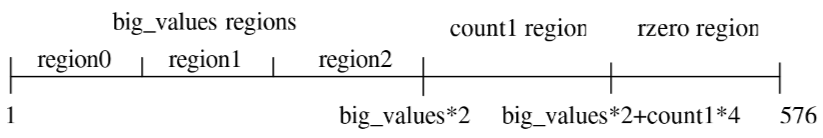
\includegraphics[width=0.8\textwidth]{big-values.png}
  \caption{big\_values felosztása}
  \label{fig:big-values}
\end{figure}

  \item [global\_gain (8-8 bit)] Kvantálás lépésköz.
  \item [scalefac\_compress (4-4 bit)] Hány bitet használjon a scalefactorok átviteléhez. Hogy az értéke alapján az első és második scalefactor group hány bitet kap az a(z) \ref{tab:scalefac-compress}. táblázatban látható.

  \begin{table}[h]
  \centering
  \footnotesize
  \begin{tabular}{|c|c|c|}
    \hline
    \textbf{scalefac\_compress} & \textbf{slen1} & \textbf{slen2} \\
    \hline
    0 & 0 & 0 \\
    \hline
    % ... (A táblázat további sorait a rövidítés miatt itt nem ismételem meg, de a kódban benne kell hagyni)
    15 & 4 & 3 \\
    \hline
  \end{tabular}
  \caption{Scalefac compress értékek}
  \label{tab:scalefac-compress}
  \end{table}

  \item [windows\_switching\_flag (1-1 bit)] Megmutatja, ha a normálon kívül másmilyen ablaktípus van használatban.
  \item [block\_type (2-2 bit)] Ha nem normál ablakot használunk, mutatja, hogy milyet. A lehetőségek a \ref{tab:block-type}. táblázatban vannak.
  
  \begin{table}[h]
  \centering
  \footnotesize
  \begin{tabular}{|c|c|}
    \hline
    \textbf{block\_type} & \textbf{window type} \\
    \hline
    00 & forbidden \\
    \hline
    01 & start \\
    \hline
    10 & 3 short windows \\
    \hline
    11 & end \\
    \hline
  \end{tabular}
  \caption{Block type értékek}
  \label{tab:block-type}
  \end{table}

  \item [mixed\_blockflag (1-1 bit)] Akkor használható, ha  a windows\_switching\_flag be van állítva. Azt jelzi, hogy más ablaktípust használunk alacsonyabb és magasabb frekvenciákon.
  \item [table\_select (10-10 bit)] Megadja milyen Huffman kódolást használjunk.
  \item [subblock\_gain (9-9 bit)] Ha windows\_switching\_flag set és block\_type == 10, akkor a gain offsetet mutatja a global gain-től.
  \item [region\_address1 (4-4 bit) region\_address2 (3-3 bit)] A spektrumot további részekre osztjuk a Huffman kódoláshoz, ezek a változók ezeknek a régióknak a kezdőcímét tartalmazzák.
  \item [preflag (1-1 bit)] További nagyfrekvenciás erősítése a kvantált mintáknak.
  \item [scalefac\_scale (1-1 bit)] A scalefactorok logaritmikusan kvantáltak a(z) \ref{tab:scalefac-scale}. táblázat szerint.
  
  \begin{table}[h]
  \centering
  \footnotesize
  \begin{tabular}{|c|c|}
    \hline
    \textbf{scalefac\_scale} & \textbf{step size} \\
    \hline
    0 & $\sqrt{2}$ \\
    \hline
    1 & 2 \\
    \hline
  \end{tabular}
  \caption{Scalefac scale értékek}
  \label{tab:scalefac-scale}
  \end{table}

  \item [count1table\_select (1-1 bit)] Huffman kódolást választ a count1 mezőben lévő értékekhez.
\end{description}

\subsubsection{Main Data}

Scalefactorokból, Huffman kódolt bitekből és ancillary data-ból áll. Az elrendezés a(z) \ref{fig:main-data-granules}. ábrán látható.
\begin{figure}[H]
  \centering
  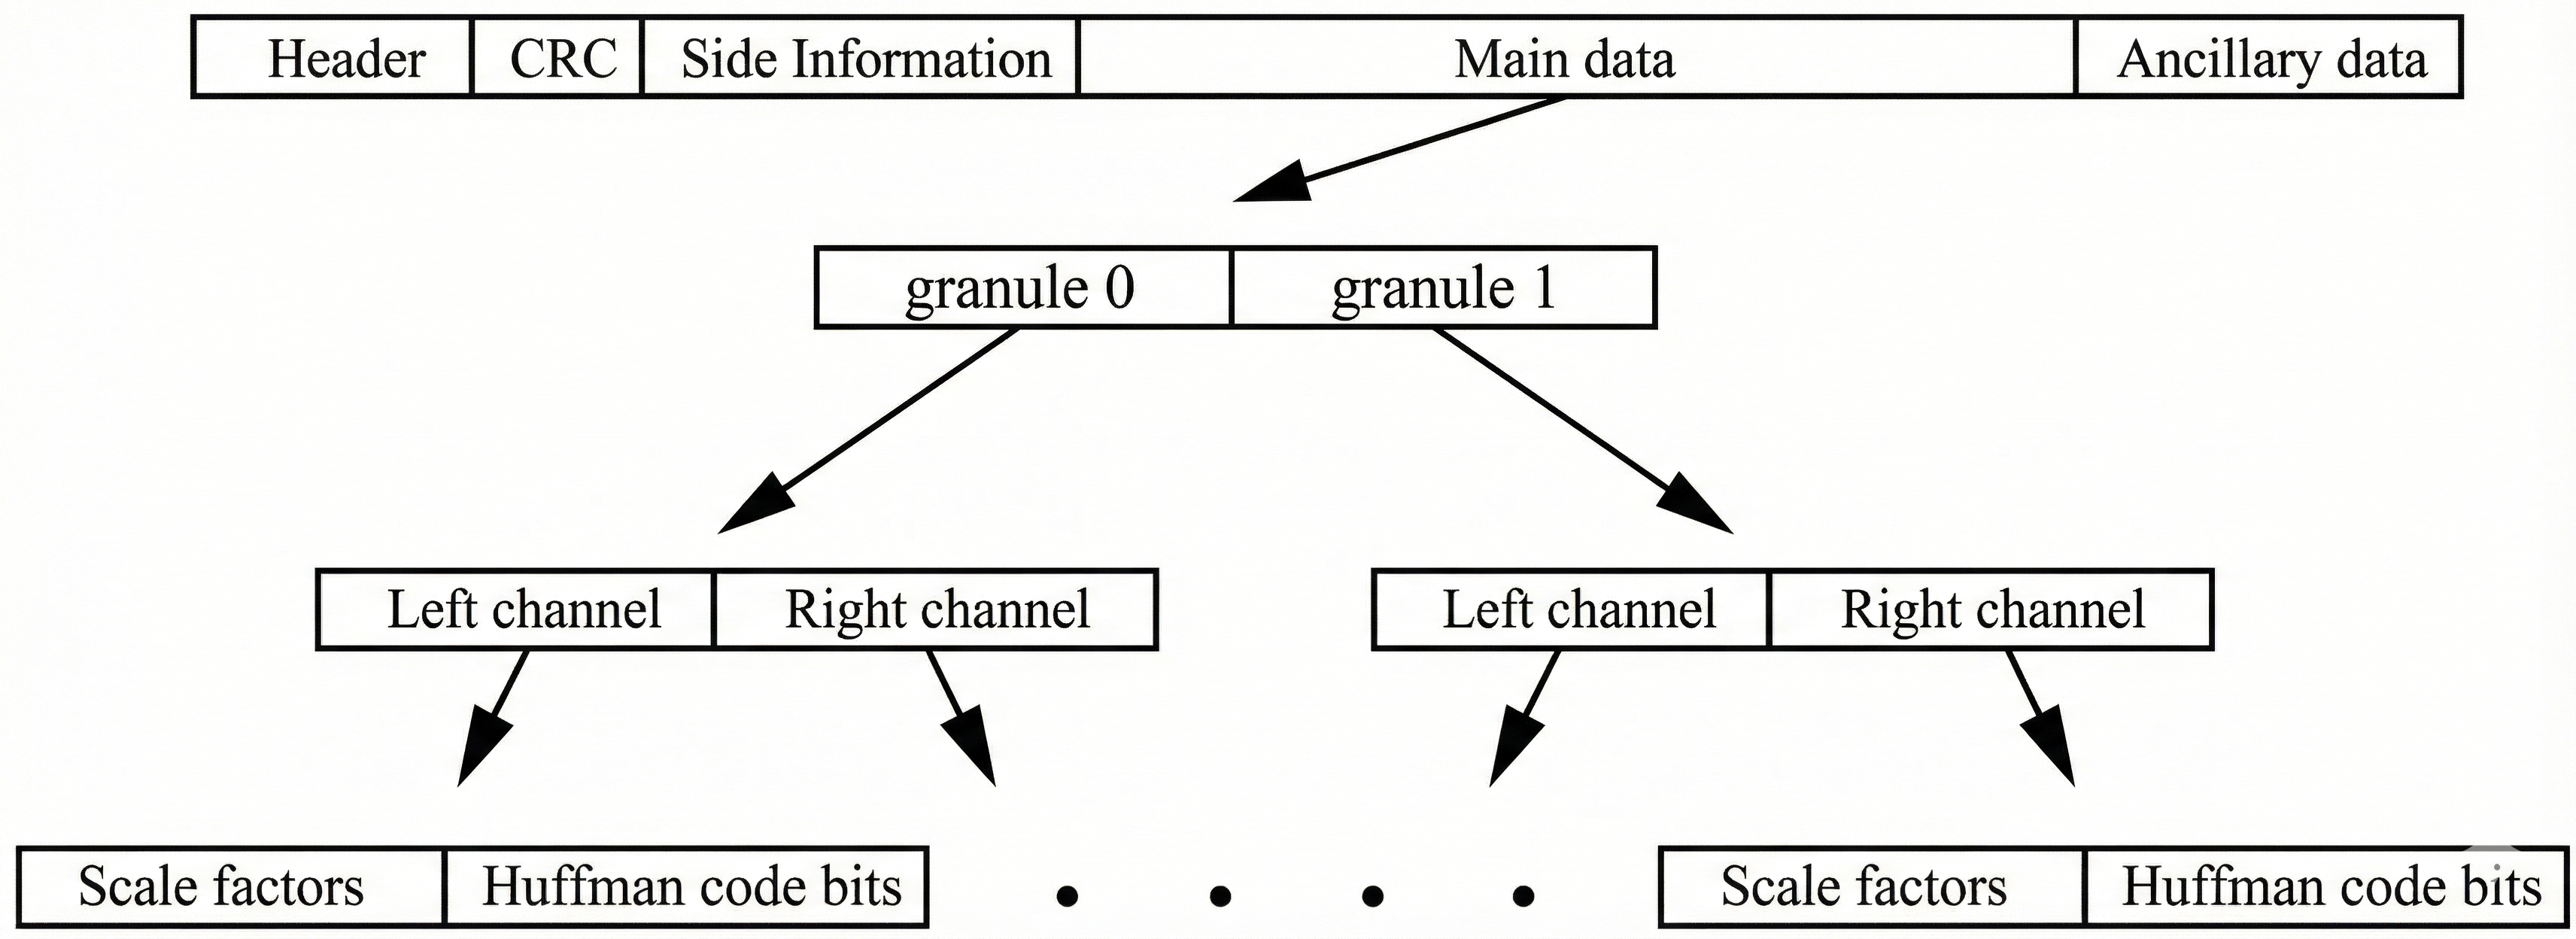
\includegraphics[width=\textwidth]{main-data-granule.png}
  \caption{Main data, granule-ok és channelek elrendezése}
  \label{fig:main-data-granules}
\end{figure}

\begin{description}
  \item [Scale factors] A céljuk, hogy redukálják a kvantálási zajt. Ha a minták egy adott scalefactor band-ben megfelelően vannak scale-elve, akkor a kvantálási zaj teljesen ki lesz maszkolva.
  \item [Huffman code bits] Itt találhatóak a Huffman kódolt bitek.
  \item [Ancillary data] Opcionális, felhasználó definiálhatja.
\end{description}


\subsection{Analysis Polyphase Filterbank}

A(z) \ref{fig:encoder-reszletes}. ábrán látható egy részletesebb blokkvázlat az encoderről. Az Analysis Polyphase Filterbankba megy a PCM input, itt az 1152 PCM minták mindegyike 32 egyenletesen eloszló frekvencia sávba lesz szétosztva.
Mivel \( f_s = 44.1 kHz \) ezért a Nyquist frekvencia \( f_{Nyquist} = 22.05 kHz \). Minden sáv \[ \frac{22050}{32} = 689.0625 Hz \] széles lesz.
Mivel minden mintát 32 subband-re osztunk, ezért az eredeti 1152-ből \( 1152*32 = 36 864 \) mintánk lesz. A folyamat végén viszont 32-vel decimálunk minden subband-et, így ismét 1152 mintánk lesz.

\begin{figure}[H]
  \centering
  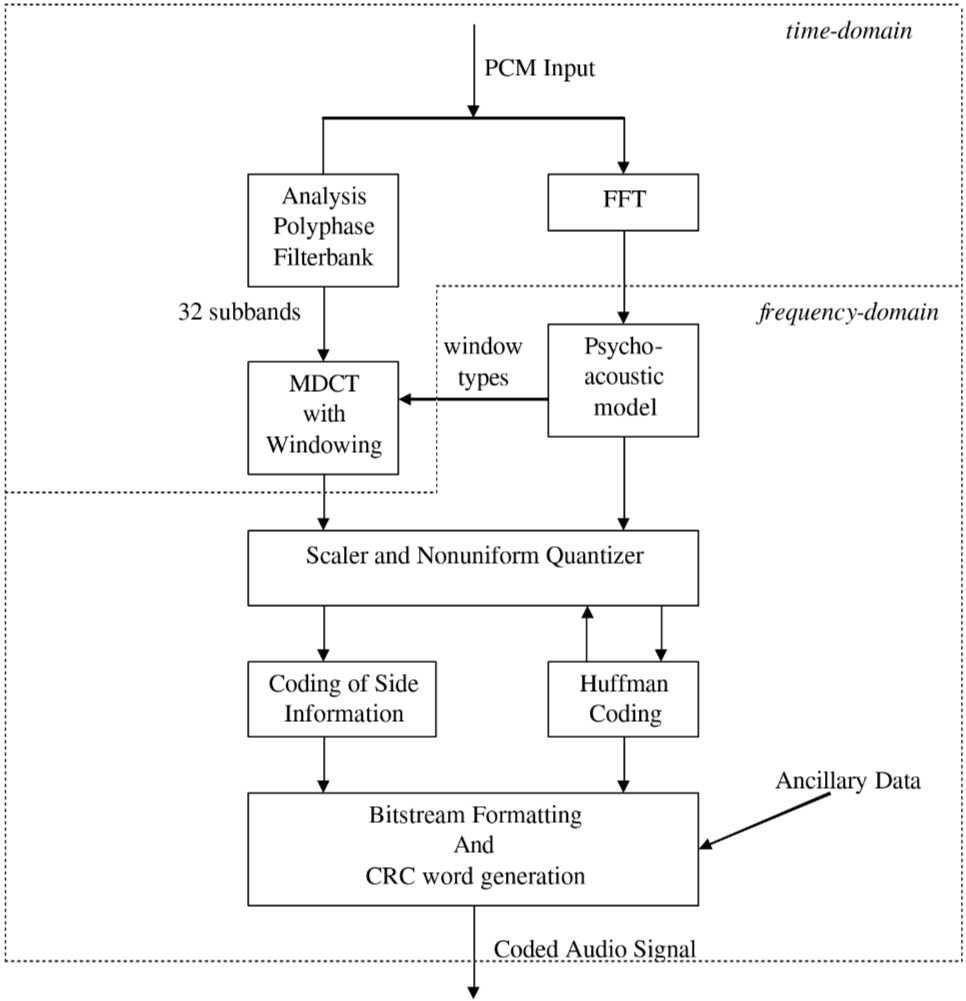
\includegraphics[width=\textwidth]{encoder-reszletes.png}
  \caption{Encoder blokkvázlat részletesebben}
  \label{fig:encoder-reszletes}
\end{figure}

\subsection{FFT tervezés}

A bejövő adatnak a spektrumát ismerünk kell a pszichoakusztív modell alkalkazásához, ezért FFT-hajtunk végre a bejövő jelen, a filterbankkal párhuzamosa.

Az FFT elvégzéséhez a Xilinx FFT IP core-ját fogom használni. Meg kell határozni, hogy az elérhető architektúrák közül melyik a legkisebb erőforrás igényű amely megfelel a célunkra. Layer III-nál két FFT-t kell párhuzamosan. Block length == window length.
\begin{description}
  \item[Short blocks] shift length = 192 samples, window length  = 256 samples
  \item[Long blocks] shift length = 576 samples, window length  = 1024 samples
\end{description}

Mivel \(f_s = 44.1 kHz\), ezért \[window\_size_1 = \frac{256}{44100} = 5.8 ms\] \[window\_size_2 = \frac{1024}{44100} = 23.2 ms\].
\[frequency\_resolution_1 = \frac{44100}{256} = 172.3 Hz\] \[frequency\_resolution_2 = \frac{44100}{1024} = 43.1 Hz\]

Látszik, hogy a kisebb ablakok jobb felbontást biztosítanak időtartományban, a hosszabb ablakok pedig frekvencia tartományban. A cél megtalálni az AMD által biztosított FFT core-nak azt a felparaméterezését, amely a lehető legkisebb erőforrás felhasználás nélkül teljesíteni tudja a követelményeket.

\textbf{Long blocks:}
\begin{itemize}
    \item Shift length: 576 samples
    \item FFT méret: 1024 points
    \item Overlap: $1024 - 576 = 448$ samples (43.75\%)
\end{itemize}

\begin{align*}
    \text{Frame } N   &: \text{samples } [0 \dots 1023] \\
    \text{Frame } N+1 &: \text{samples } [576 \dots 1599] \\
    \text{Frame } N+2 &: \text{samples } [1152 \dots 2175]
\end{align*}

\textbf{Short blocks:}
\begin{itemize}
    \item Shift length: 192 samples
    \item FFT méret: 256 points
    \item Overlap: $256 - 192 = 64$ samples (25\%)
\end{itemize}

\begin{align*}
    \text{Frame } N   &: \text{samples } [0 \dots 255] \\
    \text{Frame } N+1 &: \text{samples } [192 \dots 447] \\
    \text{Frame } N+2 &: \text{samples } [384 \dots 639] \\
\end{align*}

Hosszú ablakoknál \(\frac{576}{44100} = 13.6 ms \) idő-be telik, amíg bejön elegendő adat egy FFT végrehajtására, rövidnél  \(\frac{192}{44100} = 4.35 ms \).


A Xilinx FFT IP core-ban 4 architekrúra közül lehet választani, ezeknek az erőforrás igényét a throughput függvényében mutatja a(z) \ref{fig:fft-arch}. ábra.

\begin{figure}[H]
  \centering
  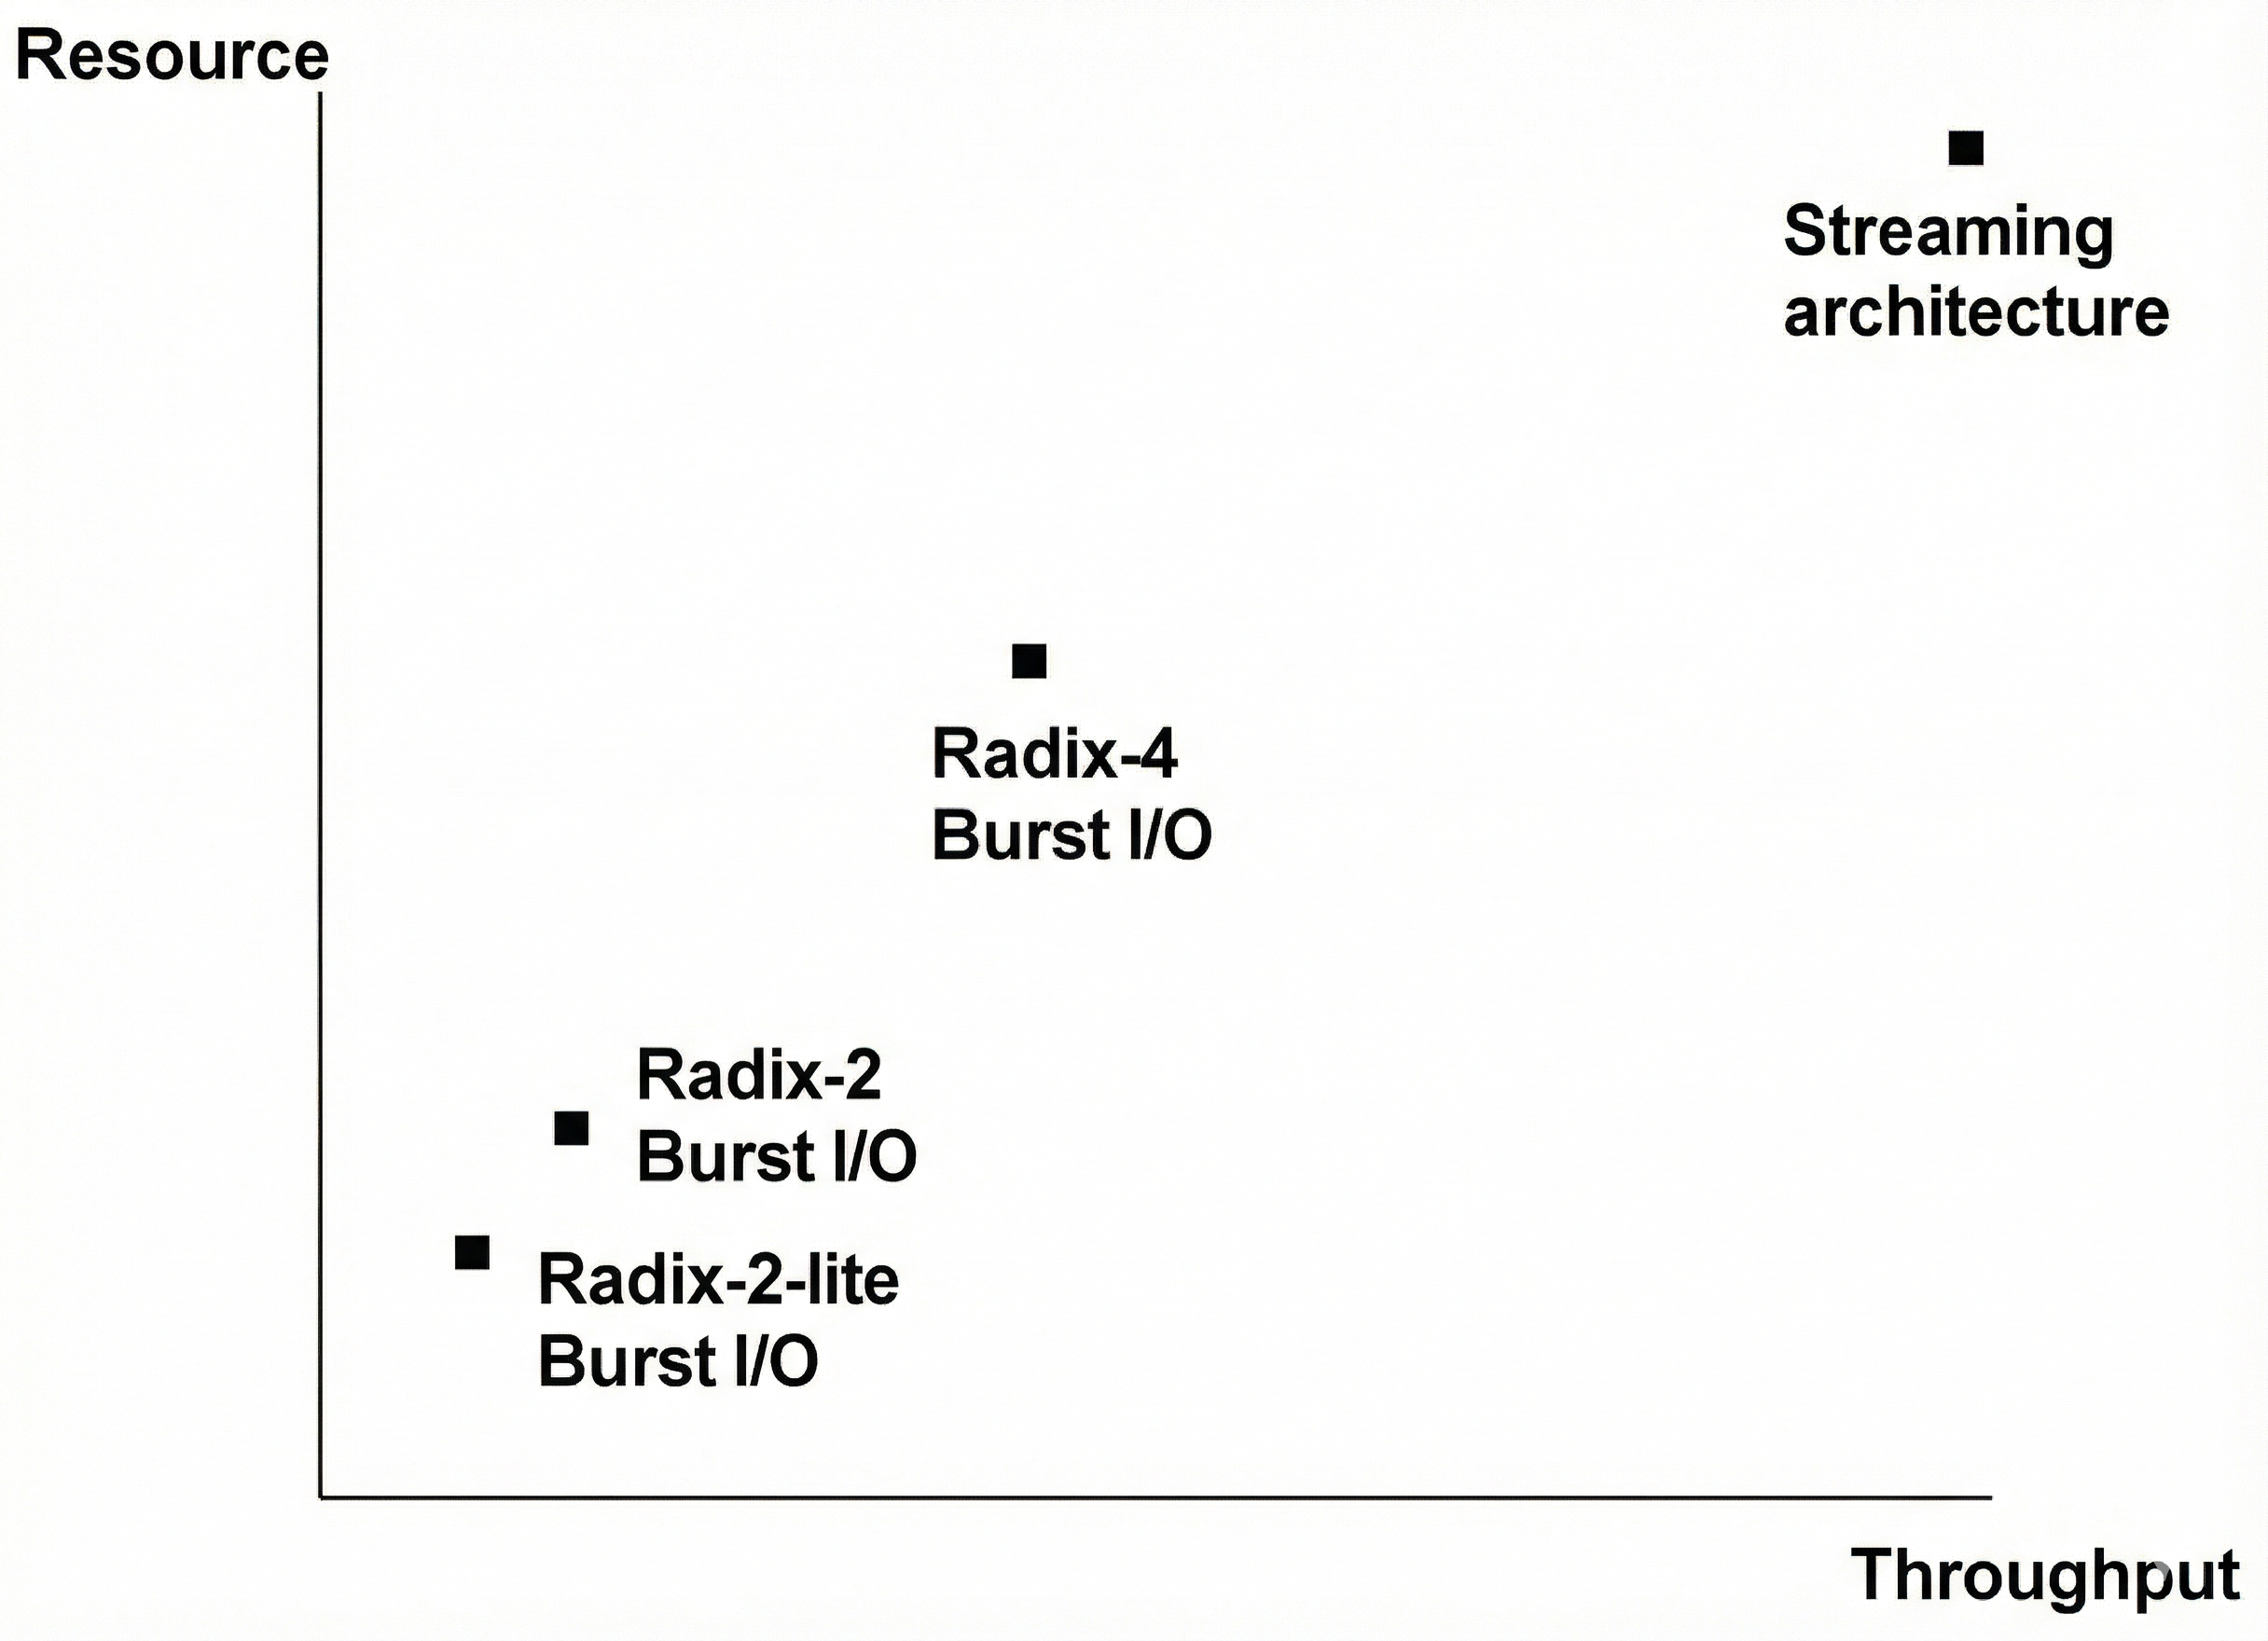
\includegraphics[width=0.6\textwidth]{architektura.png}
  \caption{Xilinx LogiCORE IP FFT architektúrák \cite{xilinx_fft}}
  \label{fig:fft-arch}
\end{figure}

A szimulációs waveform-okon a ... és ... ábrákon látszik annak az ideje, amígy kiolvasunk 256 illetve 1024 mintát és elvégezzük rajtuk az FFT-t. Mivel az 1024 pontos FFT mindig közvetlenül egy 256-os után fog jönni(576\%192 = 0), így számolni kell az IP core átkonfigurálásának az idejével is.


% -------------------------------------------------------------------------
% 7. ÉRTÉKELÉS
% -------------------------------------------------------------------------
\section{A megtervezett műszaki alkotás értékelése, továbbfejlesztési lehetőségek}
% TODO: Itt kell összefoglalni az elért eredményeket, erőforrás felhasználást, sebességet.

A tervezés során meghatároztuk az MP3 encoder alapvető paramétereit és az FPGA implementációhoz szükséges számítási kapacitást. Az FFT számítások időzítése kritikus, a számítások azt mutatják, hogy a rövid ablakok feldolgozása jelenti a szűkebb keresztmetszetet (4.35 ms).

A továbbfejlesztés iránya lehet a sztereó módok (Joint Stereo) teljeskörű implementálása és a Huffman kódolás optimalizálása hardveres gyorsítással.

% -------------------------------------------------------------------------
% 8. IRODALOMJEGYZÉK
% -------------------------------------------------------------------------
\newpage
\printbibliography

% -------------------------------------------------------------------------
% 9. MELLÉKLETEK
% -------------------------------------------------------------------------
\newpage
\appendix
\section{Mellékletek}

\subsection{Dokumentációk}
% Kapcsolási rajz, huzalozási rajz, beültetési rajz (hivatkozás a fájlokra vagy képek beszúrása)
% \includegraphics[width=\textwidth]{schematic.png}

\subsection{Forrás file-ok}
% Itt lehet hivatkozni a csatolt CD/Repo tartalmára

\subsection{Használati útmutató}
% Rövid leírás a rendszer indításáról

\end{document}
